\section{Future Work}
The experiment results suggest
significant benefits from leveraging
the ARM processor architecture for computing.
In use cases, it is possible for ARM-based processors to achieve multiples of the performance achieved by an x86 CPU 
while consuming the same amount of energy.

As an add-on to this research paper,
as well as for possible future work in
this field,
A prototype framework
for running containers in heterogeneous clusters is created.


\subsection{Prototype heterogeneous cluster}
%In order to evaluate the difficulties and the feasibility of the operation of a software on different processor architectures, a prototype is created with the use of cloud technologies. 

The prototype presents a guideline for running containers in a heterogeneous Kubernetes 
\cite{kubernetesIo} cluster,
which contains worker nodes with the x86 architecture, as well as the ARM architecture.
A graphical representation of this architecture design can be seen in Fig. 
\ref{fig:prototypeKubeCluster}.

\begin{figure}[h]
    \centering
    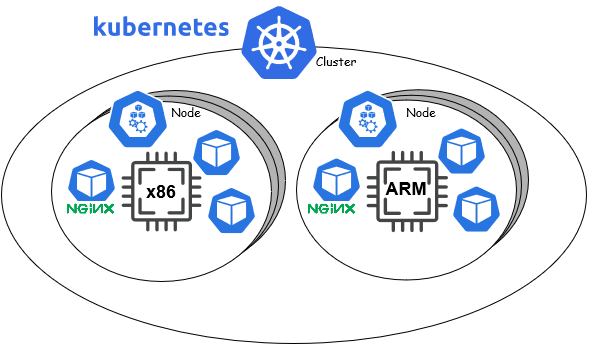
\includegraphics[width=.95\linewidth]{fig/experiment_k8s_cluster_x86_arm_v1.png}
    \caption{Prototype heterogeneous Kubernetes cluster.}
    \label{fig:prototypeKubeCluster}
\end{figure}

The virtual machines are provisioned on Amazon AWS's Elastic Compute Cloud (EC2) service 
\cite{ec2AmazonAwsWebsite}.
The AWS Marketplace 
\cite{marketplaceAmazonAwsWebsite}
offers operating system images for x86 and ARM, as well as many other machine types. 
For the prototype setup, the following Ubuntu Linux images from 
Canonical
\cite{canonicalMarketplaceAmazonAwsWebsite}
are used for x86 resp. ARM nodes:

\begin{itemize}
    \item Ubuntu 22 (Ubuntu 22.04 LTS) 
    \cite{ubuntu22amd64MarketplaceAmazonAwsWebsite}
    \item Ubuntu 22 (ARM) (Ubuntu 22.04 LTS) 
    \cite{ubuntu22arm64MarketplaceAmazonAwsWebsite}
\end{itemize}

The EC2 machines are joined together with kubeadm 
\cite{kubeadmKubernetes} 
to form a Kubernetes cluster.

Kubernetes itself automatically assigns the label "kubernetes.io/arch" to nodes 
with the value corresponding to the processor architecture.

\begin{itemize}
    \item "amd64", which equates to x86 architecture with a 64-bit instruction set.
    \item "arm64", which equates to ARM architecture with a 64-bit instruction set.
\end{itemize}

The container image nginx 
\cite{nginxDockerHub} 
from Docker Hub is used for demonstration. 
The image is offered by the maintainer in several versions for different processor architectures.
For the prototype setup, the images 
"linux/amd64" \cite{amd64ImageNginxDockerHub}
and
"linux/arm64/v8" \cite{arm64v8ImageNginxDockerHub}
in version 1.23.0
are used.

The specific images for the different processor architectures
are transparently pulled by Kubernetes to the nodes
when specifying "nginx:1.23.0".
The user does not need to specify the architecture explicitly.

Kubernetes pods can be constrained to specific nodes
based on node labels
with the concept of node affinity.
There are two types of node affinity:

\begin{itemize}
    \item \textbf{requiredDuringSchedulingIgnoredDuringExecution}: The scheduler can not schedule the Pod unless the rule is met.
    \item \textbf{preferredDuringSchedulingIgnoredDuringExecution}: The scheduler tries to find a node that meets the rule. If a matching node is not available, the scheduler still schedules the Pod.
\end{itemize}

The "requiredDuringSchedulingIgnoredDuringExecution"
affinity type can be used to constrain pods
strictly to specific nodes.

With the latter affinity type
"preferredDuringSchedulingIgnoredDuringExecution",
the key "kubernetes.io/arch" can be set to match "amd64".
This expression can be supplied a weight of e.g. "1",
while an accompanying expression can be set to match "arm64"
with a weight of e.g. "50". This results in pods
being scheduled first to arm64 nodes whenever possible,
since the weight is higher. An example configuration
in YAML format can be seen below. Long lines are
shortened and marked with "[...]".

\begin{verbatim}
affinity:
  nodeAffinity:
    requiredDuringSchedulingIgnor[...]
      nodeSelectorTerms:
      - matchExpressions:
        - key: kubernetes.io/os
          operator: In
          values:
          - linux
    preferredDuringSchedulingIgnor[...]
    - weight: 1
      preference:
        matchExpressions:
        - key: kubernetes.io/arch
          operator: In
          values:
          - amd64
    - weight: 50
      preference:
        matchExpressions:
        - key: kubernetes.io/arch
          operator: In
          values:
          - arm64
\end{verbatim}

The prototype framework introduced in this section
may be extended by other researchers
in future work. We propose the following possible topics:

\begin{itemize}
    \item Power efficiency driven workload scheduling in cluster computing.
    \item Dynamic pod scheduling and node selection in Kubernetes, based on key performance indicators and other metrics.
\end{itemize}
